\subsection{Архитектура}
    Программный комплекс позволяет производить все требуемые для решения задачи преобразования над данными, а именно:
    \begin{enumerate}
        \item получение данных из твиттера;
        \item получение данных из новостной rss-ленты;
        \item расшифровка сокращённых URL;
        \item автоматическое построение набора данных;
        \item построение моделей для методов WTMF и WTMF-G;
        \item построение рекомендаций на основе методов WTMF, WTMF-G и TF-IDF;
        \item оценка качества рекомендаций;
        \item получение результатов рекомендаций в пригодном для чтения формате;
    \end{enumerate}
    Результаты всех преобразований, за исключением оценки качества и получения рекомендаций, хранятся в специальном промежуточном
    хранилище~(побробное описания хранилища производится в разделе~\ref{sec:documentation}).

    Каждое преобразование, в общем случае, независимо от других.
    Для построения рекомендаций, необходимо выполнить цепочку преобразований.
    Примеры цепочек преобразований для получения данных, построения рекомендаций и оценки их качества приводятся ниже.
    
    Визуализация цепочек преобразований производится при помощи блок-схем~\cite{flowchart_gost}.
    Для удобства восприятия блоки действия~(изображаются прямоугольником) выделяются зелёным цветом, 
    а прочие используемые блоки, такие как ввод-вывод данных~(изображаются параллелограммом) и хранимые 
    данные~(изображаются фигурой, представляющей собой прямоугольник, в котором две противолежащие стороны 
    заменены на две одинаковые и параллельные кривые, совпадающие с секцией окружности), выделяются синим цветом.
    
    Получение данных заключается в скачивании новостей из RSS потоков и твитов, с использованием Twitter Streaming API, в течение длительного промежутка времени, с последующим помещением всех данных в промежуточное хранилище. В работе в качестве хранилища выступает python shelve.
    Получение данных в виде блок-схемы изображено на рисунке~\ref{pic:consumer_flowchart}.
    \begin{figure}[h!]
            \center
            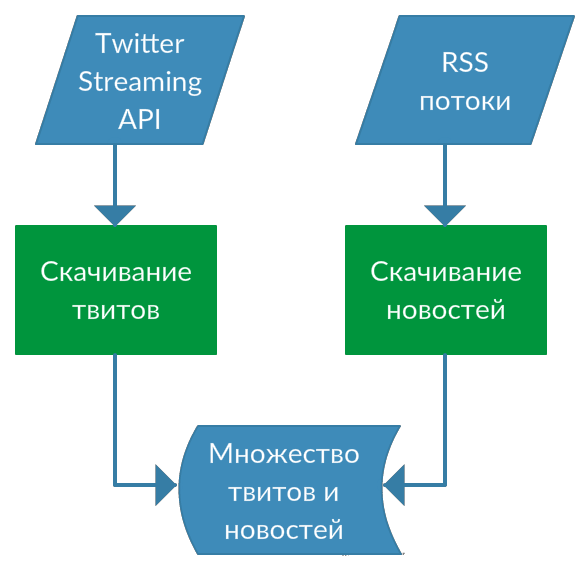
\includegraphics[scale=0.25]{twnews_consumer_flowchart.png}
            \caption{Блок-схема получения данных}
            \label{pic:consumer_flowchart}
    \end{figure}

    На основе полученного множества новостей и твитов происходит автоматическое построение набора данных. В рамках автоматического построения набора данных происходит расшифрка сокращённых URL.
    Набор данных эта структура состоящая из списка новостей и списка твитов, где для каждого твита указана ссылка на единственную новость.

    Результатом работы всех реализованных методов является сопоставление численных векторов~(векторов для сравнения) каждому обрабатываемому тексту, с помощью которых можно оценить насколько похожи любые два текста. 

    Метод TF-IDF не имеет стадии обучения модели, поэтому применяется непосредственно к набору данных и получает вектора для сравнения, для всех текстов, которые были переданы ему на вход. Получаемые вектора обладают размерностью совпадающей с размером корпуса.

    В отличие от метода TF-IDF методы WTMF и WTMF-G состоят из двух стадий: обучения и применения модели. На стадии обучения методы строят модель~(в сериализованной модели помимо самой модели содержится набор данных, на основе которого была построена модель) и получают вектора для сравнения для всех элементов набора данных. На стадии применения методы WTMF и WTMF-G на основе ранее построенной модели для произвольного множества твитов строят векторы для сравнения полученных на вход твитов и новостей из набора данных.

    На основе множества, состоящего из твитов и новостей, для каждого элемента в котором существует вектор для сравнения, строятся рекомендации.
    Рекомендации представляют собой множество твитов, к каждому из которых сопоставлен ранжированный по мере убывания схожести список новостей.

    На основе построенных рекомендаций можно как произвести оценку качества ранее использованного метода, так и получить их в виде текстового файла, который содержит информацию в пригодном для чтения формате. Оценка качества полученного метода происходит возможно, только если рекомендации были получены из набора данных.

    Процесс оценки качества различных методов рекомендаций, а также получение рекомендаций для твитов из набора данных изображён на рисунке~\ref{pic:twnews_flowchart_1}.

    \begin{figure}[h!]
            \center
            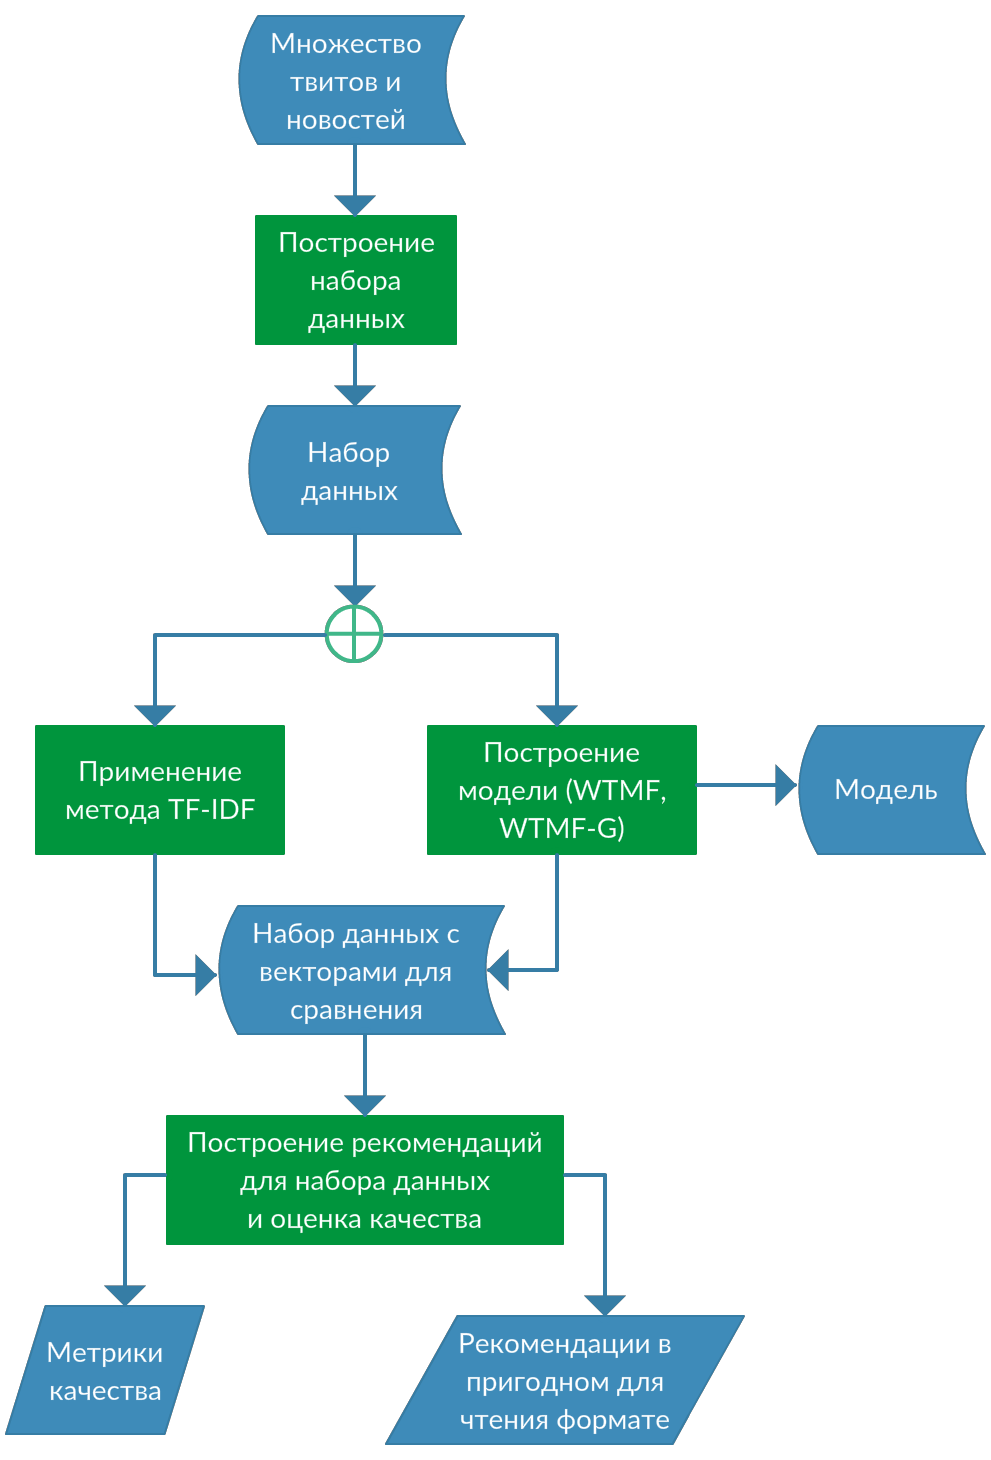
\includegraphics[scale=0.25]{twnews_flowchart_1.png}
            \caption{Блок-схема процесса оценки качества используемых методов}
            \label{pic:twnews_flowchart_1}
    \end{figure}

    Дополнительным результатом изображённого на рисунке~\ref{pic:twnews_flowchart_1} процесса является построенная модель (для методов WTMF и WTMF-G), которую можно применить на произвольное множество твитов. Процесс получения рекомендаций для произвольных твитов изображён на рисунке~~\ref{pic:twnews_flowchart_2}.
    
    \begin{figure}[h!]
            \center
            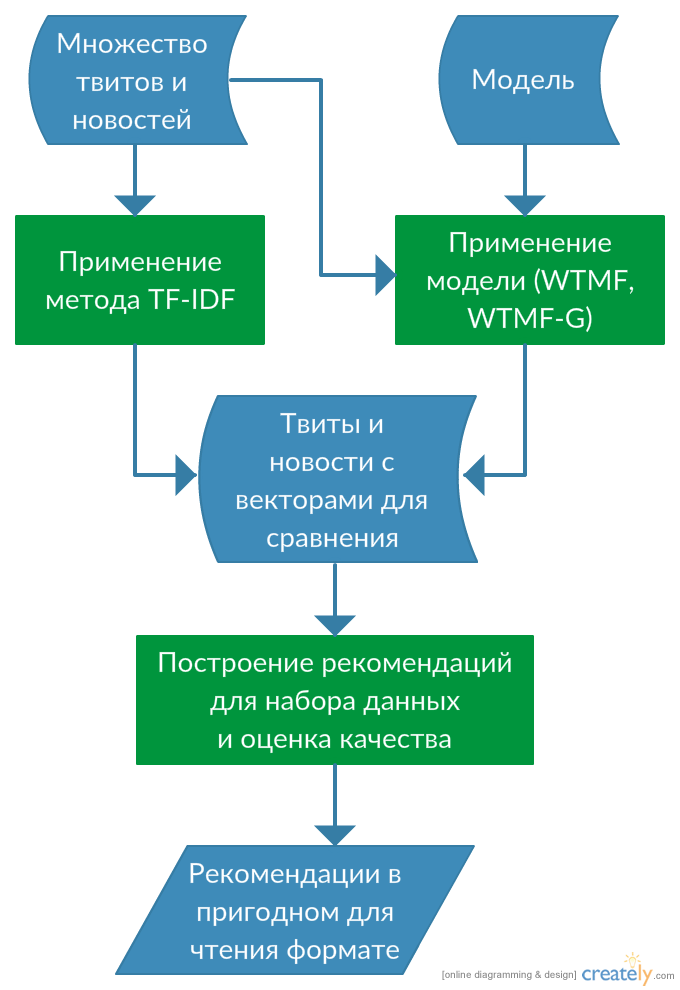
\includegraphics[scale=0.25]{twnews_flowchart_2.png}
            \caption{Блок-схема процесса получения рекомендаций для различных методов}
            \label{pic:twnews_flowchart_2}
    \end{figure}

    %\textcolor{red}{заключительный абзац}

    \clearpage



